\documentclass[12pt]{article}

\usepackage{array}
\usepackage{adjustbox}
\usepackage{amsfonts}
\usepackage{amsmath}
\usepackage{amsthm}
\usepackage{amssymb}
\usepackage{dirtytalk}
\usepackage[a4paper, total={7in, 9in}]{geometry}
\usepackage{forest}
\usepackage{geometry}
\usepackage{multirow}
\usepackage{skak}
\usepackage{tikz}
\usepackage{titling}
\usepackage{wrapfig}
\usepackage{xcolor}

\usetikzlibrary{patterns}

\def\multichoose#1#2{\ensuremath{\left(\kern-.3em\left(\genfrac{}{}{0pt}{}{#1}{#2}\right)\kern-.3em\right)}}

\usetikzlibrary{decorations.pathreplacing}
\usetikzlibrary{patterns}

\pgfdeclarepatternformonly{bigger north west lines}{\pgfqpoint{-2pt}{-2pt}}{\pgfqpoint{8pt}{8pt}}{\pgfqpoint{6pt}{6pt}}%
{
  \pgfsetlinewidth{1pt}
  \pgfpathmoveto{\pgfqpoint{0pt}{6pt}}
  \pgfpathlineto{\pgfqpoint{6.2pt}{-0.2pt}}
  \pgfusepath{stroke}
}

\newcommand*{\Scale}[2][4]{\scalebox{#1}{$#2$}}
\newcommand*{\SetHeight}[2]{\resizebox{!}{#1}{$#2$}}

\begin{document}
\pagenumbering{gobble}

\title{Math 142 Study Guide}
\date{2016-10-06}
\author{David Alves}

\begin{center}
\large \thetitle \\
by \theauthor \\
\end{center}
\section*{Notation \& Basics}
\newcommand{\termtable}[1]{
    \def\arraystretch{1.75}
    \begin{tabular}{ r p{28em} }
    #1
    \end{tabular}
}
\newcommand{\term}[1]{\textbf{#1}&}

\termtable{
    \term{set} A collection of elements where the order doesn't matter and every element is distinct (You can't have two elements that are equal to each other)\\
    \term{list or $k-$tuple} A collection of elements $(a_1, a_2, \ldots, a_k)$ where the order matters and duplicates are allowed. For example $(1, 2)$ is different from $(2,1)$ and $(1,1)$ is a valid list.\\
    \term{$a \in A$} $a$ is an element of the set $A$\\
    \term{$a \notin A$} $a$ is \textbf{not} an element of the set $A$\\
    \term{$|S|$} The number of elements in a set $S$ (\emph{cardinality} of $S$)\\
    \term{$A \cap B$} The \emph{intersection} of $A$ and $B$, namely the set of elements that are in both $A$ and $B$\\
    \term{$A \cup B$} The \emph{union} of $A$ and $B$, namely the set of elements that are either in $A$, in $B$, or in both\\
    \term{$A \subset B$} $A$ is a \emph{subset} of $B$, meaning $A$ contains only elements that are in $B$. (Note for this class $A$ and $B$ can be equal, we are not using \say{proper subset})\\
    \term{$A \times B$} The \emph{cartesian product} of sets $A$ and $B$, namely the set of every possible list $(a, b)$ where $a \in A$ and $b \in B$. Example: $A=\{1,2\}, B=\{3,4\},A \times B = \{(1, 3), (1, 4), (2, 3), (2, 4)\}$\\
    \term{$\emptyset$ or $\{\}$} The empty set, the set with no elements\\
    \term{disjoint} Sets $A$ and $B$ are disjoint if they have no elements in common, meaning $A \cap B = \emptyset$\\
    \term{$\binom{n}{k}$} Number of subsets of size $k$ in a set of $n$ items, $\frac{n!}{k!(n-k)!}$\\

    \term{domain} The set of values that can go into a function. By definition a function can be applied to every element of the domain\\
    \term{codomain} That set of values that can come out of a function\\
    \term{injective} Every element in the codomain is hit at \textbf{most} once\\
    \term{surjective} Every element in the codomain is hit at \textbf{least} once\\
    \term{bijective} Every element of the codomain is hit \textbf{exactly} once (both injective and surjective)\\
    \term{$f : A \rightarrow B$} A function $f$ with domain $A$ and codomain $B$\\
    \term{$[n]$} The set of integers $\{1, 2, \ldots, n-1, n\}$\\
}

\section*{Twelvefold Way with Balls and Bins}
\newcommand{\twelvecell}[2]{
    \begin{center}
        \minsizebox*{!}{.6cm}{$\displaystyle #1$}
    \end{center}
    #2
}
\newcommand{\twelverow}[1]{
    \centering #1
}

\newcommand{\finishrow}[0]{
    \medskip\\
    \hline
}

\def\arraystretch{1.2}
\lapbox[\width]{-.8cm}{
\begin{tabular}{ m{1.2cm}m{5.2cm}m{5.2cm}m{5.2cm}c }
     & \large\centering General           & \large\centering Injective                  & \large\centering Surjective&\\
     & \small\centering No restrictions & \small\centering At \textbf{most} one ball per bin & \small\centering At \textbf{least} one ball per bin&\\
    \hline
    
    
    \twelverow{$a$ balls\\(dist.)\bigskip\\$b$ bins\\ (dist.)} & 
    \twelvecell{b^a}{There are $b$ choices for each ball, so by the product principle there are $b^a$ total configurations.}& 
    \twelvecell{\prod_{i=0}^{a-1}b-i}{There are $b$ choices for the first ball, $b~-~1$ choices for the second ball (since it can't go in the same one), $b-2$ choices for the third, etc. ($\prod$ is like $\sum$ except you multiply the terms instead of adding them)} &
    \twelvecell{S(a,b)b!}{There are $S(a,b)$ ways to put distinguishable balls into indistinguishable bins by definition, and then $b!$ ways to label the bins after you have placed the balls.}
    \finishrow
    
    \twelverow{$a$ balls\\(indist.)\bigskip\\$b$ bins\\ (dist.)} & 
    \twelvecell{\multichoose{b}{a}=\binom{a+b-1}{a}}{Use $\star$ for a ball and $\vert$ for a divider between bins. There are $b-1$ dividers needed so you have a sequence of $a+b-1$ elements of which $a$ are balls, giving $\binom{a+b-1}{a}$. For example, $(0, 0, 3, 1)$ is $\vert\vert\star\star\star\vert\star$}&
    \twelvecell{\binom{b}{a}}{Number of ways to pick a subset of size $a$ from a set of size $b$. (We are picking $a$ of the bins to contain a single ball while the rest remain empty).}&
    \twelvecell{\binom{a-1}{a-b}}{Use the same stars-and-bars encoding as for general, except since each bin must have one ball, we can leave it out of the encoding. For example, $(3,1,2)$ is encoded as $\star\star\vert\vert\star$}
    \finishrow 
 
    \twelverow{$a$ balls\\(dist.)\bigskip\\$b$ bins\\ (indist.)} & 
    \twelvecell{\sum_{i=0}^{b} S(a,i)}{$S(a,i)$ is the number of ways to put $a$ balls into $i$ bins such that all bins contain at least one ball. Sum over all values of $i$ to get the total number of ways to fill $b$ bins without the \say{all bins used} requirement}&
    \twelvecell{
        \begin{aligned}    
            b\geq a: 1\\
            b<a: 0
        \end{aligned}
    }{One way if there are enough bins, otherwise zero}&
    \twelvecell{S(a,b)}{$S(a,b)$ is defined to be the number of ways to place $a$ distinguishable balls into $b$ indistinguishable bins. Note that this is also the number of ways to partition a set with $a$ elements into $b$ groups.}
    \finishrow  
 
    \twelverow{$a$ balls\\(indist.)\bigskip\\$b$ bins\\ (indist.)} &  
    \twelvecell{\sum_{i=0}^{b} P(a,i)}{$P(a,i)$ is the number of ways to put $a$ balls into $i$ bins such that all bins contain at least one ball. We then sum over all values of $i$ from 0 to $b$ to get the total number of ways to fill $b$ bins without the \say{all bins used} requirement}&
    \twelvecell{
        \begin{aligned}    
            b\geq a: 1\\
            b < a: 0
        \end{aligned}
    }{One way if there are enough bins, otherwise zero}&
    \twelvecell{P(a,b)}{This is defined to be the number of ways to place $a$ indistinguishable balls into $b$ indistinguishable bins. Note that this is also the number of ways to partition an integer $a$ into the sum of $b$ integers and the number of Young Diagrams with $a$ boxes and $b$ rows.}
\end{tabular}
}
\section*{Equivalence Relations \& Partitions}
\termtable{
    \term{relation} A relation is a subset of $A \times B$. A \say{relation on $A$} is a subset of $A\times A$\\
    \term{equivalence relation} An equivalence relation is a relation that satisfies three properties:
        \begin{itemize}
        \item Reflexive: All pairs of the form $(a, a)$ in $A\times B$ are present in the relation
        \item Symmetric: If $(a, b)$ is in the relation, then $(b, a)$ must be in the equivalence relation.
        \item Transitive: If $(a, b)$ and $(b, c)$ are in the relation, then $(a, c)$ must be in the relation.
        \end{itemize}\\
    \term{partition} A partition of a set $S$ is a set of disjoint subsets of $S$ such that the union of those subsets is equal to $S$. For example, $\{\{1,2,4\},\{3,5\}\}$ is a partition of $[5]$ because $\{1,2,4\} \cup \{3,5\} = [5]$ and $\{1,2,4\} \cap \{3,5\} = \emptyset$.
}

\pagebreak
\section*{Pascal's Triangle \& Binomial Theorem}
\begin{center}
\begin{tikzpicture}[
    scale=1,
    tcancel/.append style={draw=#1, cross out, inner sep=1pt}
]
\node at ( 0, 0) {1};
\node at (-1,-1) {1};
\node at ( 1,-1) {1};
\node at (-2,-2) {1};
\node at ( 0,-2) {2};
\node at ( 2,-2) {1};
\node at (-3,-3) {1};
\node at (-1,-3) {3};
\node at ( 1,-3) {3};
\node at ( 3,-3) {1};
\node at ( 0, -4.5) {$\vdots$};
\node at (-6, -6) {1};
\node at (-4.5, -6) {$\ldots$};
\node at (-3, -6) (up2l) {$\binom{n-1}{k-2}$};
\node at (-1, -6) (up1l) {$\binom{n-1}{k-1}$};
\node at ( 1, -6) (up1r) {$\binom{n-1}{k}$};
\node at ( 3, -6) (up2r) {$\binom{n-1}{k+1}$};
\node at ( 4.5, -6) {$\ldots$};
\node at ( 6, -6) {1};
\node at (-7, -7) {1};
\node at (-5.5, -7) {$\ldots$};
\node at (-4, -7) (main2l) {$\binom{n}{k-2}$};
\node at (-2, -7) (main1l) {$\binom{n}{k-1}$};
\node at ( 0, -7) (maincc)  {$\binom{n}{k}$};
\node at ( 0, -6.5) {+};
\node at ( 2, -7) (main1r){$\binom{n}{k+1}$};
\node at ( 4, -7) (main2r){$\binom{n}{k+2}$};
\node at (5.5, -7) {$\ldots$};
\node at ( 7, -7) {1};
%\draw [->, thick] (up2r)--(main2r);
%\draw [->, thick] (up2r)--(main1r);
%\draw [->, thick] (up1r)--(main1r);
\draw [->, thick] (up1r)--(maincc);
\draw [->, thick] (up1l)--(maincc);
%\draw [->, thick] (up1l)--(main1l);
%\draw [->, thick] (up2l)--(main1l);
%\draw [->, thick] (up2l)--(main2l);
\end{tikzpicture}
\end{center}
\subsection*{Pascal's Triangle Properties}
\begin{itemize}
\item $k^{\text{th}}$ element of $n^{\text{th}}$ row has value $\binom{n}{k}$
\item Each item is the sum of the two above it: $\binom{n-1}{k-1} + \binom{n-1}{k} = \binom{n}{k}$
\item Sum of $n^{\text{th}}$ row $\sum_{k=0}^{n}\binom{n}{k}=2^n$
\item Sum of even-indexed terms in row $n$ = Sum of odd-indexed terms in row $n$ = Sum of terms in row $n-1$.
\end{itemize}
\subsection*{Binomial Theorem}
\begin{align*}
    (x+y)^n &= \sum_{k=0}^n \binom{n}{k}x^{n-k}y^k\\
    &= \binom{n}{0}x^n + \binom{n}{1}x^{n-1}y + \binom{n}{2}x^{n-2}y^2 + \ldots\\
\end{align*}

Note that if you set $x=y=1$, this says that the sum of the $n^{\text{th}}$ row  of Pascal's Triangle is $2^n$.
\pagebreak
\section*{Catalan Numbers}
\begin{align*}
    C_n &= 1, 1, 2, 5, 14, 42, \ldots\\
    C_n &= \frac{1}{n+1}\binom{2n}{n}\\
    C_{n+1} &= \sum_{k=0}^{n} C_kC_{n-k}\\
\end{align*}
$C_n$ is the number of paths from $(0, 0)$ to $(0, 2n)$ using only diagonally up and diagonally down moves and without crossing X-axis:
\begin{center}
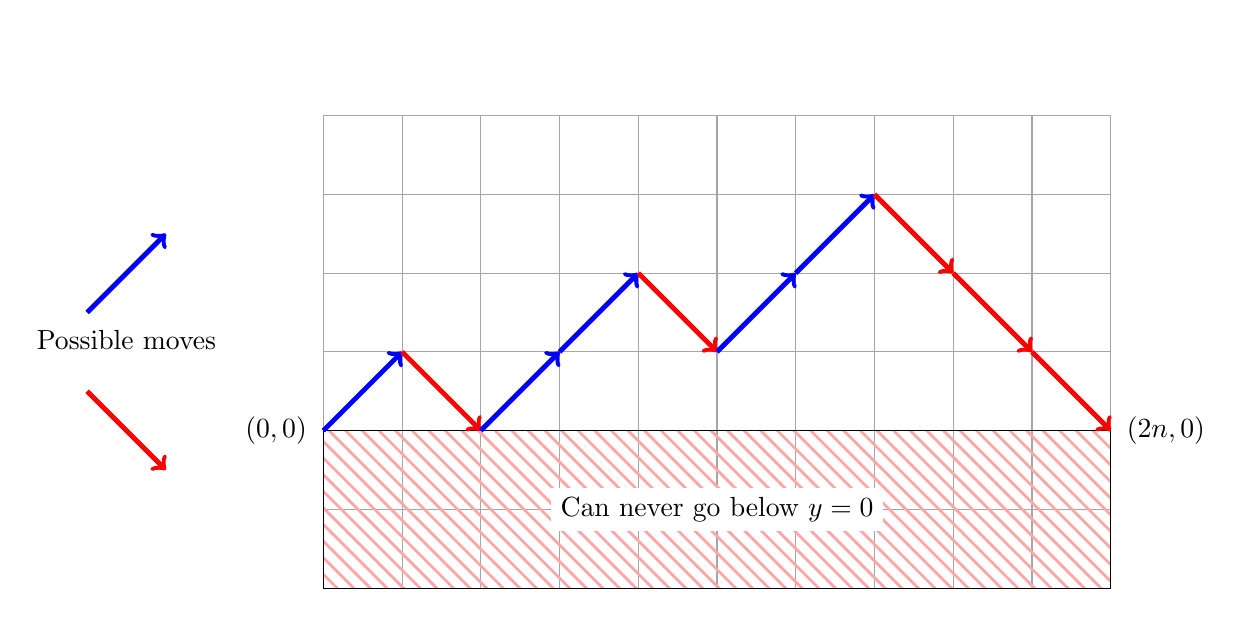
\begin{tikzpicture}
\draw[step=1.0,black,thin,color=black,opacity=.35] (-5,-2) grid (5,4);
\node (S) at (-5, 0) {};
\node (E) at (5, 0) {};
\node (T) at (-5, 5) {};

\draw[pattern=bigger north west lines, pattern color=red!35] (-5,0) rectangle (5,-2) node [midway,fill=white] {Can never go below $y=0$};


\draw [->,line width=1.75,blue] (-8,1.5) -- (-7,2.5) node[midway, black, yshift=-2.4em] {Possible moves};
\draw [->,line width=1.75,red]  (-8,0.5) -- (-7,-.5);

\draw [->,line width=1.75,blue] (-5,0) -- (-4,1);
\draw [->,line width=1.75,red] (-4,1) -- (-3,0);
\draw [->,line width=1.75,blue] (-3,0) -- (-2,1);
\draw [->,line width=1.75,blue] (-2,1) -- (-1,2);
\draw [->,line width=1.75,red] (-1,2) -- (0,1);
\draw [->,line width=1.75,blue] (0,1) -- (1,2);
\draw [->,line width=1.75,blue] (1,2) -- (2,3);
\draw [->,line width=1.75,red] (2,3) -- (3,2);
\draw [->,line width=1.75,red] (3,2) -- (4,1);
\draw [->,line width=1.75,red] (4,1) -- (5,0);
\node [black] at (-5.6,0) {$(0,0)$};
\node [black] at (5.7,0) {$(2n,0)$};
\end{tikzpicture}
\end{center}

$C_n$ is also the number of distinct trees with $n$ nodes (where nodes are read left to right, so for example reflection symmetry doesn't count).
\pagebreak


\section*{Principle of Inclusion-Exclusion}

The union of $n$ sets $S_1, S_2, \ldots, S_n$ can be computed in terms of intersections of those sets. This is handy when intersections are easier to count than unions.

Example for $n=4:$
\newcommand{\dlist}[1]{S_{#1}}
\begin{multline}\label{eq:ps6_3_1}
    |\dlist{1} \cup \dlist{2} \cup \dlist{3} \cup \dlist{4}| = |\dlist{1}| + |\dlist{2}| + |\dlist{3}| + |\dlist{4}|\\ 
    -|\dlist{1} \cap \dlist{2}| - |\dlist{1} \cap \dlist{3}| - |\dlist{1} \cap \dlist{4}| - |\dlist{2} \cap \dlist{3}| - |\dlist{2} \cap \dlist{4}| - |\dlist{3} \cap \dlist{4}|\\
    +|\dlist{1} \cap \dlist{2} \cap \dlist{3}| + |\dlist{1} \cap \dlist{2} \cap \dlist{4}| + |\dlist{1} \cap \dlist{3} \cap \dlist{4}| + |\dlist{2} \cap \dlist{3} \cap \dlist{4}|\\
    -|\dlist{1} \cap \dlist{2} \cap \dlist{3} \cap \dlist{4}|
\end{multline}

%\[xC^2(x)-C(x) + 1 = 0\]
\section*{Generating Functions}
Coming soon...

\end{document}
